% Use the following line _only_ if you're still using LaTeX 2.09.
%\documentstyle[icml2015,epsf,natbib]{article}
% If you rely on Latex2e packages, like most moden people use this:
\documentclass{article}

% use Times
\usepackage{times}
% For figures
\usepackage{graphicx} % more modern
%\usepackage{epsfig} % less modern
\usepackage{subfigure} 

% For citations
\usepackage{natbib}

% For algorithms
\usepackage{algorithm}
\usepackage{algorithmic}

% As of 2011, we use the hyperref package to produce hyperlinks in the
% resulting PDF.  If this breaks your system, please commend out the
% following usepackage line and replace \usepackage{icml2015} with
% \usepackage[nohyperref]{icml2015} above.
\usepackage{hyperref}

% Packages hyperref and algorithmic misbehave sometimes.  We can fix
% this with the following command.
\newcommand{\theHalgorithm}{\arabic{algorithm}}

% Employ the following version of the ``usepackage'' statement for
% submitting the draft version of the paper for review.  This will set
% the note in the first column to ``Under review.  Do not distribute.''
%\usepackage{icml2015} 

% Employ this version of the ``usepackage'' statement after the paper has
% been accepted, when creating the final version.  This will set the
% note in the first column to ``Proceedings of the...''
\usepackage[accepted]{icml2015}



% The \icmltitle you define below is probably too long as a header.
% Therefore, a short form for the running title is supplied here:
\icmltitlerunning{Volleyball Match Summarization}

\begin{document} 

\twocolumn[
\icmltitle{Generating Natural Language Summaries of Volleyball Matches}

% It is OKAY to include author information, even for blind
% submissions: the style file will automatically remove it for you
% unless you've provided the [accepted] option to the icml2015
% package.
\icmlauthor{Michael Drews}{mdrews@hawk.iit.edu}
\icmladdress{Illinois Institute of Technology,
           10 W 35th St, Chicago, IL 60616}


% You may provide any keywords that you 
% find helpful for describing your paper; these are used to populate 
% the "keywords" metadata in the PDF but will not be shown in the document
\icmlkeywords{CS 597, volleyball, NLP, NLG}

\vskip 0.3in
]

\begin{abstract} 
With a big focus of the field of natural language generation on generating tweets and short snippets of text, this project aims to increase the scope of generation by creating news articles that summarize volleyball matches. This data-to-text program will be given the box score and play-by-play log of a single match and will generate a pretty article that highlights the players that did particularly well and summarizes each of the sets within the match. A data-driven template approach will be used, in which the language used in historical articles will influence the content of the templates and the characteristics of the current set will be compared to historical matches to determine which template sentences to use. 
\end{abstract} 

\section{Introduction}

The game of volleyball is a popular international sport, especially in the United States at the collegiate level. Universities that have competitive intercollegiate programs spend a lot of time practicing and scouting to improve their chance at success. In order to properly scout other teams, it's important for quantitative stats to be taken of their matches. As a result, for all games at the NCAA level, there's an official team of statisticians at each game that keeps track of player and team stats as well as play-by-play information of how each point ends. All of this data is then publicly available on the NCAA website\footnote{For example: https://stats.ncaa.org/game/index/4485145}. Universities also typically have reporters that will write articles following each of the matches that are also available online. 

For the schools that don't have dedicated reporters or the intramural leagues that have stats but no articles, it could be beneficial to have a program that takes those stats as input and generates a summarizing article with a data-to-text algorithm. 

The task of generating text from a non-linguistic input (Natural Language Generation) has a long history with different types of approaches. Recently, data-driven deep neural network architectures have been used to map from input data to a linguistic output when sufficient amount of data is present. Among other techniques, using templates as the foundation of the algorithm is a viable approach that offers fine-tuned modification of the language and a guarantee that ungrammatical sentences aren't generated. 

For this project, the historical articles and stats from Illinois Tech volleyball matches will be used in 
a template-based NLP application that will create a new article with a match's box score and play-by-play log as the input.

\section{Data Collection}

All of the data is publicly available from the Illinois Tech Athletics website. However, it's all within HTML documents, so the biggest challenge in accumulating the data was parsing through all of the websites and creating and populating the data structures.  Here are examples of the articles and stats pages for a particular Illinois Tech volleyball match:

\textbf{http://www.illinoistechathletics.com/sports/mvball/2017-18/releases/20180112x11gbc}

\textbf{http://www.illinoistechathletics.com/sports/mvball/2017-18/boxscores/20180112\_1ei7.xml}

\textbf{http://www.illinoistechathletics.com/sports/mvball/2017-18/boxscores/20180112\_1ei7.xml?view=plays}

\subsection{Historical Data}

In order to take a data-driven approach to generating the templates, the text from 121 historical articles was gathered. First all of the schedule webpages had to be crawled to compile a list of the URLs for all of the articles and stat webpages. Then requests were made to those URLs to retrieve the source HTML. Each article contains the following main sections: 
\begin{itemize}
\item Title
\item Introduction
\item How It Happened
\item Scarlet Hawk Standouts
\item Stats To Know
\item Up Next
\end{itemize}

The gathered sentences were split up based on the section they were from so that there was a corpus of sentences from all of the Titles, a corpus of sentences from all of the Introductions, etc. 

In addition to the language from the historical articles, the corresponding play-by-play logs were also parsed and gathered. For the play-by-play logs, each row shows which team won the point, how the point was won, which player was responsible for winning the point, and the score up to that point. Those values were parsed from each row and a list of python namedtuples was used to store these logs. Additionally, for each set in the match, the associated play-by-play data was vectorized using the point differential after each point to create a vector of length 10. In total there were 571 sets and each of those vectors were clustered into 5 clusters. 

There were a few challenges with gathering the historical data. In particular, on days in which two games were played, the article actually summarized both matches. So it had to be determined which match each section was referring to so that the appropriate stats and play-by-play data could be linked to those sentences. Moreover, some coreference resolution was required as oftentimes school nick names or acronyms would be used and it had to be linked back to the same opponent. There also were some discrepancies between articles, which made it difficult to run a single program that was compatible with all of the articles. Overall, this was one of the more difficult phases of the project and a lot of consideration was put into properly collecting the data and linking it back to the appropriate team.

\subsection{Current Data}
When generating a new article, all that's known beforehand is what's available from the box score and play-by-play log. The box score contains the stats for each player and team totals and ultimately a python dictionary is created that maps a player's name to a second dictionary that maps the name of a particular stat to its actual value for that player. The play-by-play log is parsed in the same way as it was for the historical data and is again vectorized for each set in the match. 

\section{Play-by-play Classification}
\subsection{Vectorization}
In order to mathematically compare the play-by-play logs in such a way that sets with similar language would have high similarity, the logs had to be vectorized in a particular way. Ultimately, the point differential from the logs is used to create the vector. The point differential is a single integer that states how many points Illinois Tech is leading or trailing by and the list of these numbers over the course of a match is a good indication of how the match progressed. For example, if all of the point differentials are positive with an increasing slope, Illinois Tech led the whole time and dominated the match. If the point differentials fluctuate around 0, it was a very close back-and-forth set. Importantly, the language used to describe each set is heavily dependent upon the way the set played out and how well Illinois Tech performed. So two sets with similar point differential vectors will likely be described using similar language. 

One challenge is that the number of points in a set varies, since the set ends as soon as one team hits at least 25 points and is leading by 2, so the vectors are a different length for each set. To reduce the vectors to a constant length, a list of 10 lists is created and the point differentials are split up as evenly as possible within those 10 sublists while preserving their order. Then the average of each of those sublists is computed to get a vector of length 10 that contains the average point differential for the first 10\% of the set, then the average point differential for the next 10\% of the match, and so on. 

These constant length vectors were created for each of the 571 historical sets and then were clustered into five clusters using a k-means clustering algorithm provided by the python sklearn package. With these clusters, a new play-by-play vector can be classified to see which cluster it is closest to and the chosen templates for the set summary ultimately depend on which cluster the vector ends up in. The cluster centroids can be seen in the following figure:
\begin{figure}[ht]
\begin{center}
\centerline{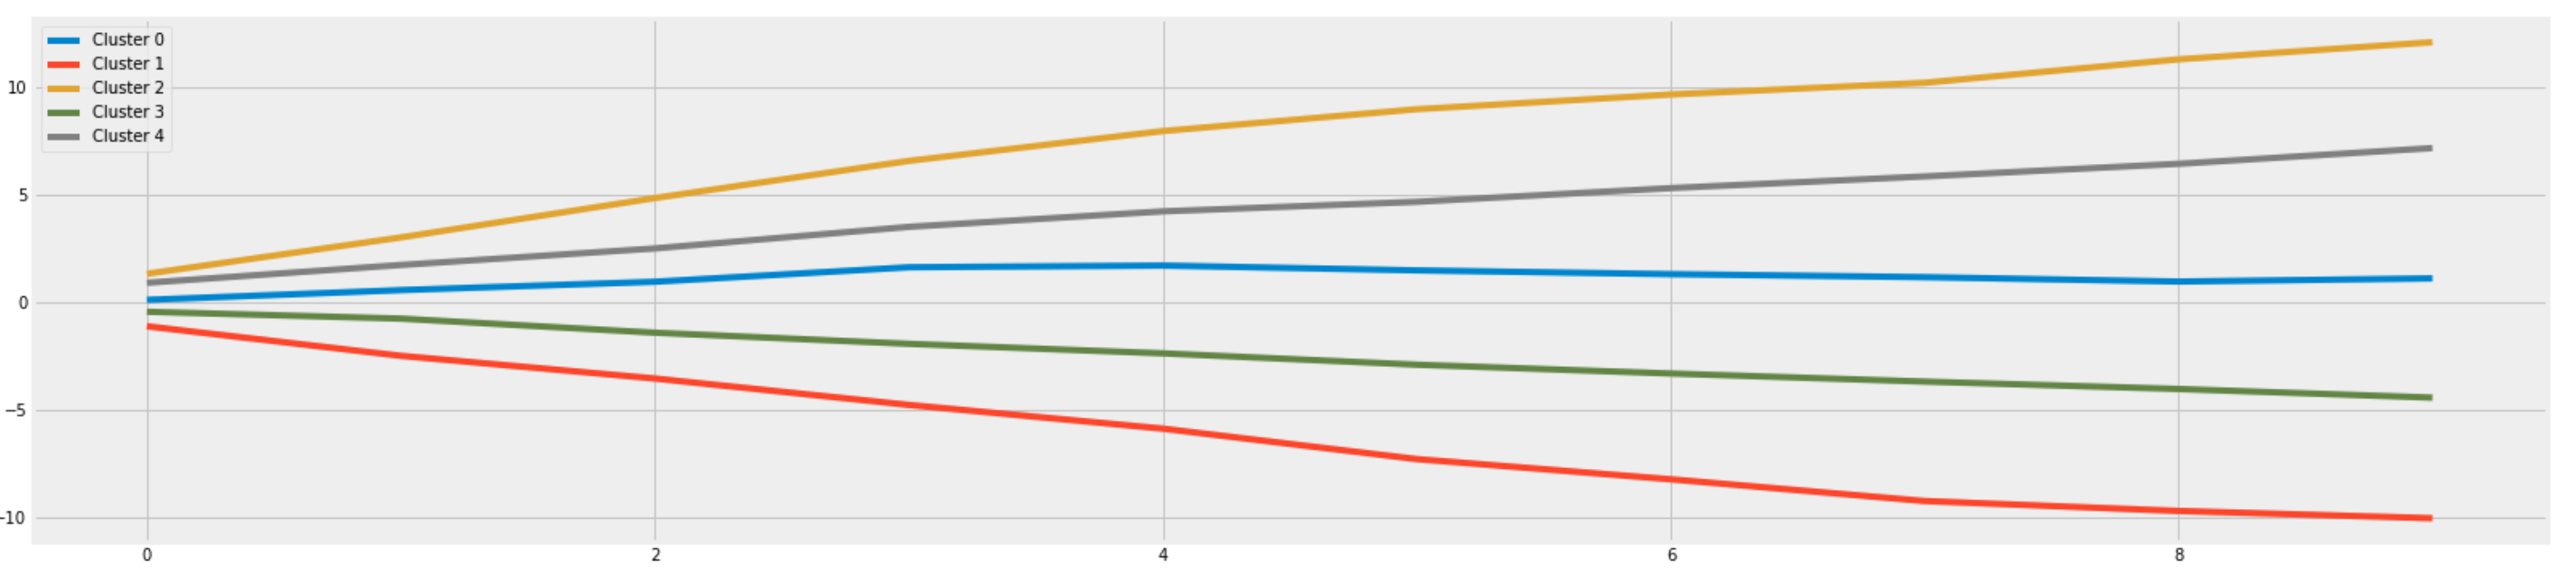
\includegraphics[width=\columnwidth]{clusters}}
\caption{Line plots for each of the cluster centroids for the play-by-play log clustering.}
\label{clusters}
\end{center}
\end{figure} 
\section{Templates}
The template generation was split up based on the previously mentioned sections of the article; each section will have its own set of templates with different policies for choosing and completing the sentences. The template sentences contain tags that get replaced by the corresponding value. Some tags refer to a general category like \texttt{lose-verb}, which could ultimately be replaced by one of many verbs like \texttt{beats}, \texttt{tops}, or \texttt{defeats}. In this sense, the templates are similar to a context free grammar in which some tags are non-terminal symbols that eventually produce one of many terminal strings. This is used for adding adjectives, noun phrases, and verb phrases to the templates without have to write entirely unique sentences for each possible combination. One sample template for the article's title is as follows:
\begin{verbatim}
<GENDER>'s Volleyball <good-verb> <OPP>
\end{verbatim}

From this example template, the \texttt{<GENDER>} tag will be replaced appropriately with \texttt{Men} or \texttt{Women}, the \texttt{<good-verb>} tag can be replaced with one of many verbs like \texttt{Shuts Out} or \texttt{Cruises Past}, and the \texttt{<OPP>} tag is replaced with the name of the opposing school. This template sentence in particular is only chosen if Illinois Tech wins the game. In fact, the title templates are split up into two partitions: one list of sentences if they won and another if they lost. From looking at the historical titles, the language in the title mainly depended on the match results and not so much on the details of the match. So a sentence is chosen from the appropriate partition and then the sentence is created by filling in the tags. 

Finally, one historical article's HTML file was downloaded and stripped of its content, like the sentences, player names, stats, etc. Unique tags were then added to the HTML tags that contained the original content. This template HTML file then serves as the basis for the generated article, as it contains all of the formatting from the original article and it has easily identifiable tags that are ultimately filled in with the newly generated content.

\section{Article Generation}
To summarize the procedure, the player and team stats are first saved in a dictionary by scraping through the HTML webpage at the given URL. Additional necessary information is retrieved from the box score, such as which team is the home team, which is the away, the name of the opposing school, the location of the match, and more. Then the play-by-play logs from the HTML page are saved in a list of namedtuples.  Some brief preprocessing is performed on the data to determine whether Illinois Tech won the match, how many sets were played, and what the score for each of those sets was. Next, the play-by-play log for each set is vectorized using the previously described method and then classified to get a cluster assignment for each set. 

With the previous steps completed, the sentences can now be generated. The process is split up into each of the six aforementioned categories, as they each have their own template of sentences. Each section has a corresponding method that is responsible for returning a string or a list of strings that then are added to the base HTML page at the appropriate location.  

\section{Results}
Articles generated by this program can be found in the following directory:
\begin{verbatim}
/master/src/article_generation/results
\end{verbatim}

There are two articles that describe the same winning match and another two that describe the same losing match.

\section{Discussion}

Following the conclusion of this project, there were a few key successes that made a big impact on the outcome. The first is the process of vectorizing the play-by-play data. There are many ways to cluster time-series data of varying lengths, but the approach used of creating a constant length vector is both straightforward to implement and easy to intuitively grasp. Each feature in the vector is a quantitative measure of how well Illinois Tech performed for that section of the set. The length of 10 was somewhat arbitrarily chosen, and this value can be modified to change how fine-tuned you want the vectors to be. A small number will take the average over longer durations of the match, whereas a high number will allow for features that correspond to short segments of the match. 

Furthermore, treating the templates roughly as a context free grammar makes it much easier to add new sentences and non-terminals to the sentences. For example, if it was desired to add a new noun phrase for when IIT lost, it can just be added as an additional terminal symbol to the existing tag. And since multiple non-terminal tags can be used in the same sentence, the total number of possible sentences increases by the product of how many terminal symbols each non-terminal produces. So rather than having two possible sentences  

\begin{verbatim}
IIT easily beat their opponent
\end{verbatim}
\begin{verbatim}
IIT crushed their opponent
\end{verbatim}

these can be combined to 

\begin{verbatim}
IIT <winning-verb-phrase> their opponent
\end{verbatim}
where
\begin{verbatim}
<winning-verb-phrase> -> easily beat
<winning-verb-phrase> -> crushed
\end{verbatim}

As previously stated, this simplifies the modification of the templates, by allowing additions to the non-terminal symbols to affect multiple possible sentences.

Finally, reusing the existing HTML and CSS of the Illinois Tech articles was a good way to create a legitimate presentation for the generated content, as opposed to, say, just returning a list of possible sentences in a .txt file.

There are still a few shortcomings, though, that could use some work in the future. The templates as they are could use some improvement, as they're still relatively simple. Fortunately this is a straightforward process and a big gain in output variance can be achieved by adding just a few more sentences. One potential addition could be a production along the lines of
\begin{verbatim}
S -> S <conj> S
<conj> -> but, while, whereas
\end{verbatim}

Compound sentences are possible with the current template, but they're "hardcoded" into the base template sentence. By making it a probabilistic possibility to combine multiple sentences, it could allow for a good mix between simple and compound sentences.

Improving the number of possible sentences will help with the second issue of redundancy. Right now it's possible for sentences to be reused and it can really hurt the flow of the summaries. One quick fix would be to randomly select sentences without replacement, which isn't currently done. That, in addition to adding more sentences, will go a long way in increasing the variance of the generated sentences. 

There's also room for improvement with the set summary templates in the clusters that represent close sets. Currently there are three classes of sentences: "easy win", "win", and "loss". The sets that belong in the middle cluster whose features fluctuate around a point differential of 0 could be much better described if they had a class of template sentences of their own with the appropriate language for a very close set. Right now the set summaries aren't necessarily incorrect for the close sets, but these close sets are arguably the most exciting and the summaries could benefit from having templates specific to those situations.

Finally, wrapping the project within a graphical user interface will make it much easier to change the URLs and view the generated article. It could potentially even generate multiple articles and allow the user to pick and chose the parts they like to create one ultimate article. Since the main idea behind this project was to create a program that can be easily demonstrated to others, this step would really help achieve that goal.

Overall, having started from scratch with a limited time frame, I'm very happy with the program and what it can become with some further work. There were moments of discouragement and worry when initial approaches didn't pan out as anticipated, but learning from those attempts and modifying the approach until arriving at the program as it currently stands was a very rewarding experience. 

\nocite{survey}
\nocite{pass}

\bibliography{report}
\bibliographystyle{icml2015}

\end{document} 